\section{Protocolo In-Band}
\label{sec:ana_inband}

En esta sección, se tomará la decisión de seleccionar el protocolo de control in-band que se utilizará en el proyecto. Después de una cuidadosa evaluación de las opciones disponibles, se ha decidido utilizar el protocolo IoTorii \cite{rojas2021outperforming}, basado en el enfoque de enrutamiento jerárquico, como la solución más adecuada. Esta elección se respalda por el hecho de que el autor del proyecto ha participado activamente en el desarrollo del protocolo IoTorii, lo que garantiza un conocimiento profundo y una experiencia práctica en su implementación.\\
\\
El protocolo IoTorii ofrece una serie de ventajas significativas para el control in-band en entornos de \gls{iot}. Su enfoque jerárquico de etiquetado permite una gestión eficiente y escalable de la red, al tiempo que proporciona una mayor flexibilidad y adaptabilidad a las necesidades específicas del proyecto. Además, IoTorii ha sido probado y validado en diversas situaciones y escenarios, demostrando su eficacia y confiabilidad en la práctica.\\
\\
En este contexto, se ha tomado la decisión de hacer uso de los caminos generados por el protocolo IoTorii, donde cada nodo de la red posee rutas distintas para alcanzar el nodo raíz de la topología. En el caso de este proyecto, el nodo raíz se designará como el controlador (o el nodo que brinda acceso al controlador). Por lo tanto, la innovación radica en la implementación de IoTorii en un entorno de redes definidas por software (SDN).La integración de IoTorii con el entorno SDN permitirá aprovechar las capacidades y ventajas de ambos enfoques. La combinación de la eficiencia y escalabilidad jerárquica de IoTorii con la flexibilidad y el control centralizado de SDN ofrece un enfoque prometedor para el desarrollo y la gestión de redes \gls{iot}. Este enfoque innovador proporcionará una base sólida para llevar a cabo el proyecto y permitirá explorar nuevas posibilidades y mejoras en el ámbito del control in-band para entornos de \gls{iot}.

\subsection{Protocolo IoTorii}

El protocolo IoTorii fue diseñado para trabajar en redes de baja capacidad en entornos \gls{iot}, tratando de solventar carencias de otros protocolos del mismo ámbito como \gls{rpl}, basándose en dos principios: (1) Intercambiar menos mensajes y reducir el tamaño de las tablas de rutas, y (2) Ofrecer resiliencia a través de caminos de \textit{back-up}, con una exploración inicial relativamente rápida. Dichos principios básicos tratan de impactar sobre el consumo y la robustez de las redes de baja capacidad, factores clave en este tipo de redes.


\subsubsection{Operativa del protocolo IoTorii}

El objetivo de IoTorii es dar cada nodo de la red por lo menos una etiqueta jerárquica, en adelante \gls{hlm}, para establecer una jerarquía en la topología. Otra forma de verlo puede ser ver la jerarquía como un árbol que se va ramificando, y está enraizado en el nodo que actúa como \textit{root}. Las \gls{hlm} tratan de proveer de más significado a las MACs convencionales. IoTorii está basado en el protocolo GA3 \cite{rojas2017ga3}, el cual trataba de buscar el mismo etiquetado jerárquico pero en redes cableadas de Data Centers. El principio de estas etiquetas está basado en una revisión del estandar \texttt{ieee802} que se hizo para dar cabida al uso de direcciones MAC mejoradas para el reenvío de paquetes en red.\\
\\
El proceso de la difusión de dichas etiquetas se pueden ver en la figura \ref{fig:iotorii-operation}. El primer paso es establecer en la topología quien va a actuar como nodo \textit{root}, este caso según se puede apreciar es el nodo \texttt{A}. Este nodo será el encargado de iniciar todo el proceso de asignación de etiquetas en la topología. La asignación de etiquetas empezará desde el \textit{root} haciendo uso de un mensaje de tipo \textit{SetHLMAC}, el cual consiste en mandar la \gls{hlm} del remitente más un sufijo que se asociará al vecino. Pero, ¿A qué consideramos vecino? La condición de vecino se da cuando dos nodos se encuentran en rango de cobertura, y se han notificado entre ellos de su presencia mediante un mensaje de tipo \textit{Hello}. Dicho mensaje es una trama vacía donde solo anuncian su dirección MAC real. \\
\\
Un símil en la vida real podría verse como cuando una nueva familia llega al vecindario y va casa por casa presentándose, ``¡Hola somos nuevos aquí {\DejaSans 😃}! Acabamos de llegar al vecindario, nos hemos mudado a la casa de enfrente". Sin embargo, no te sueles presentar con todas las personas del vecindario, solo con los vecinos más cercanos, pporqueno te interesa que todos sepan de ti, solo aquellos con los que vayas a tener relación por cercanía.\\
\\
\begin{figure}[ht!]
    \centering
    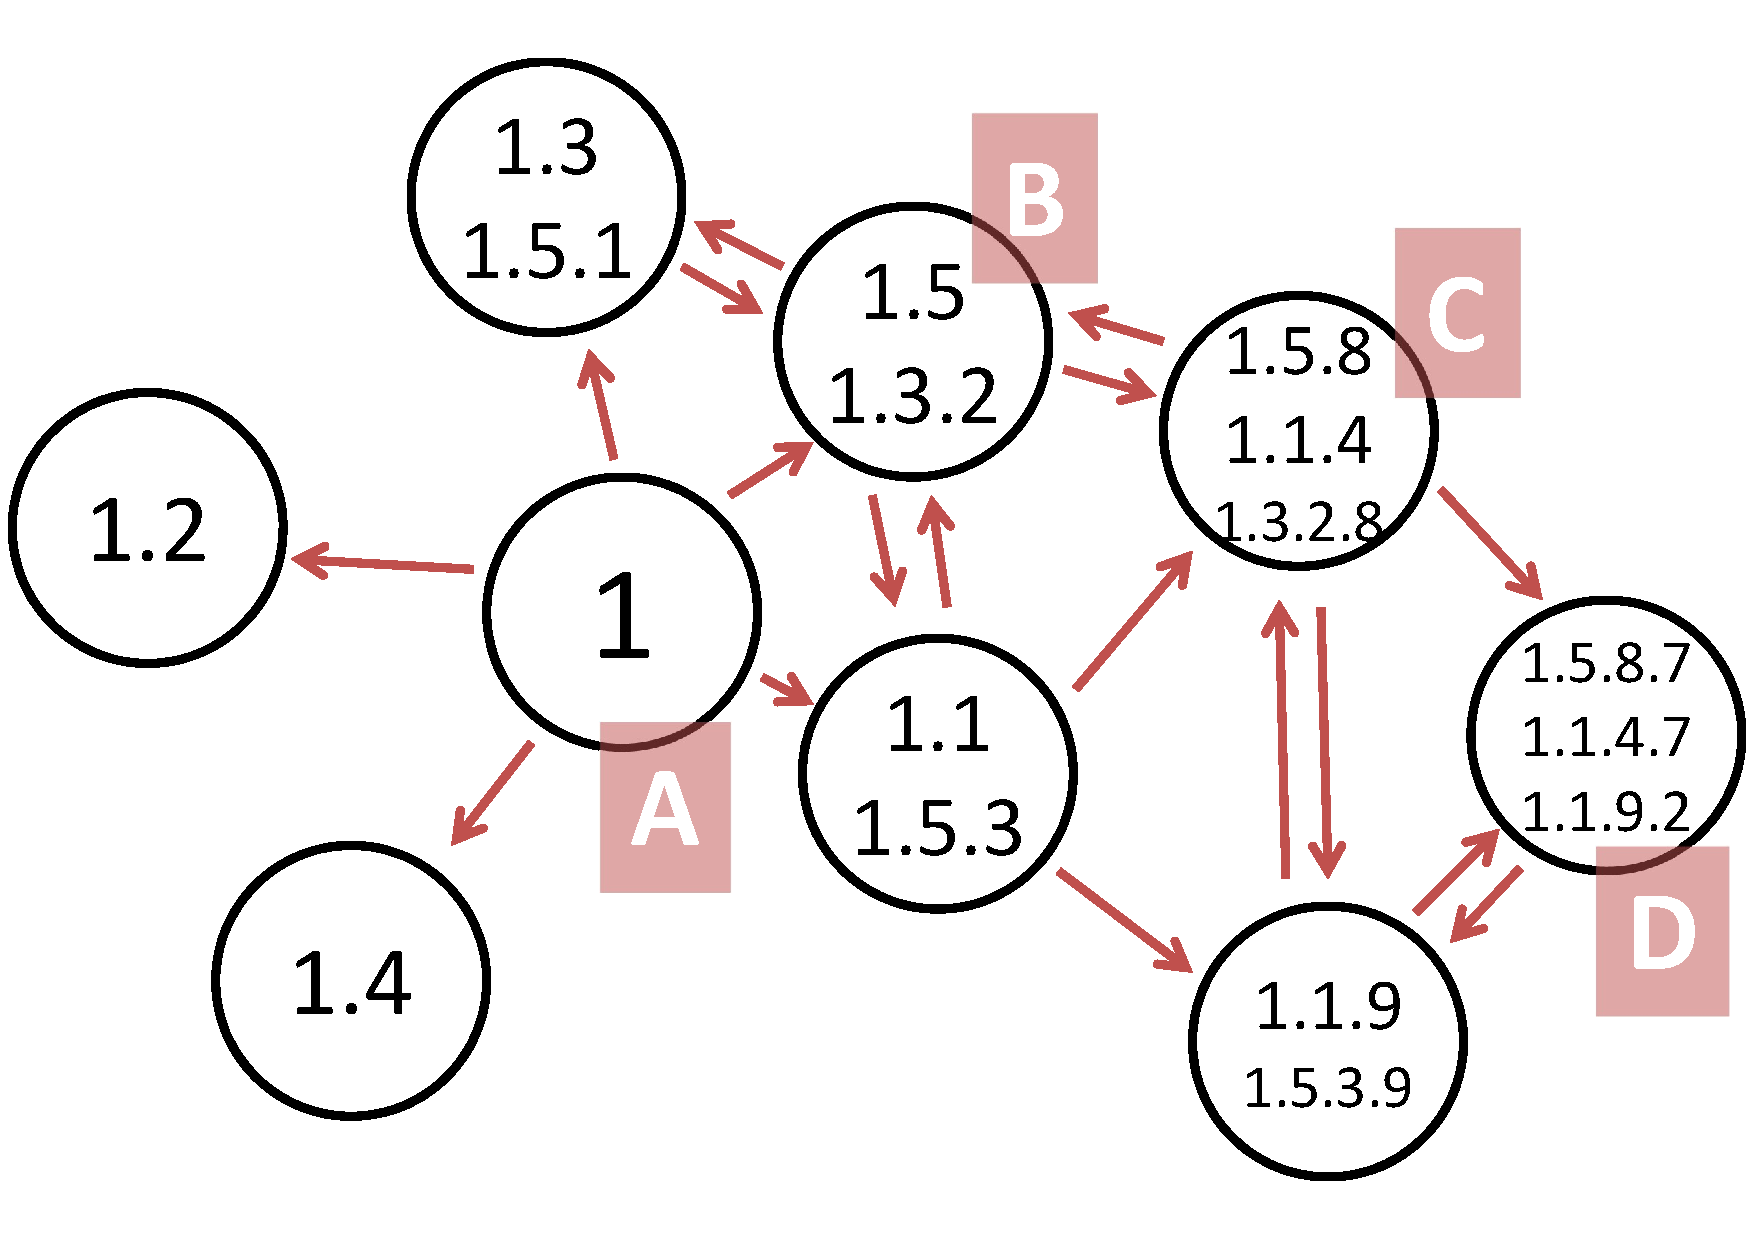
\includegraphics[width=\textwidth]{archivos/img/analisis/iotorii-operation.pdf}
    \caption{Operativa del protocolo de IoTorii \cite{rojas2021outperforming}}
    \label{fig:iotorii-operation}
\end{figure}



\begin{algorithm}[ht!]
    \SetAlgoLined
    %\KwResult{Write here the result }
    % initialization\;
    send \textit{Hello}\;
    \While{frame received}{
        %instructions\;
        \uIf{Hello}{
            \eIf{MAC not in Hello table}{
                assign unique \textit{suffix}\;
                save tuple \{\textit{MAC,suffix}\}\;
                \If{root node}{
                    create \textit{SetHLMAC} with HLMAC=1\;
                    \For{each tuple in Hello table}{
                        add tuple to \textit{SetHLMAC}\;
                    }
                    broadcast \textit{SetHLMAC}\;
                }
            }{
                discard\;
            }
        }
        \uElseIf{SetHLMAC}{
            \eIf{HLMAC (or prefix) not in HLMAC table}{
                save HLMAC in \textit{HLMAC table}\;
                create \textit{SetHLMAC} with received HLMAC\;
                \For{each tuple in Hello table}{
                    add tuple to \textit{SetHLMAC}\;
                }
                broadcast \textit{SetHLMAC}\;
            }{
                discard\;
            }
        }
        \Else{
            discard\;
        }
    }
    \caption{Assignment of HLMACs in IoTorii}
    \label{iotorii-alg}
\end{algorithm}

\begin{sidewaysfigure}
    \centering
    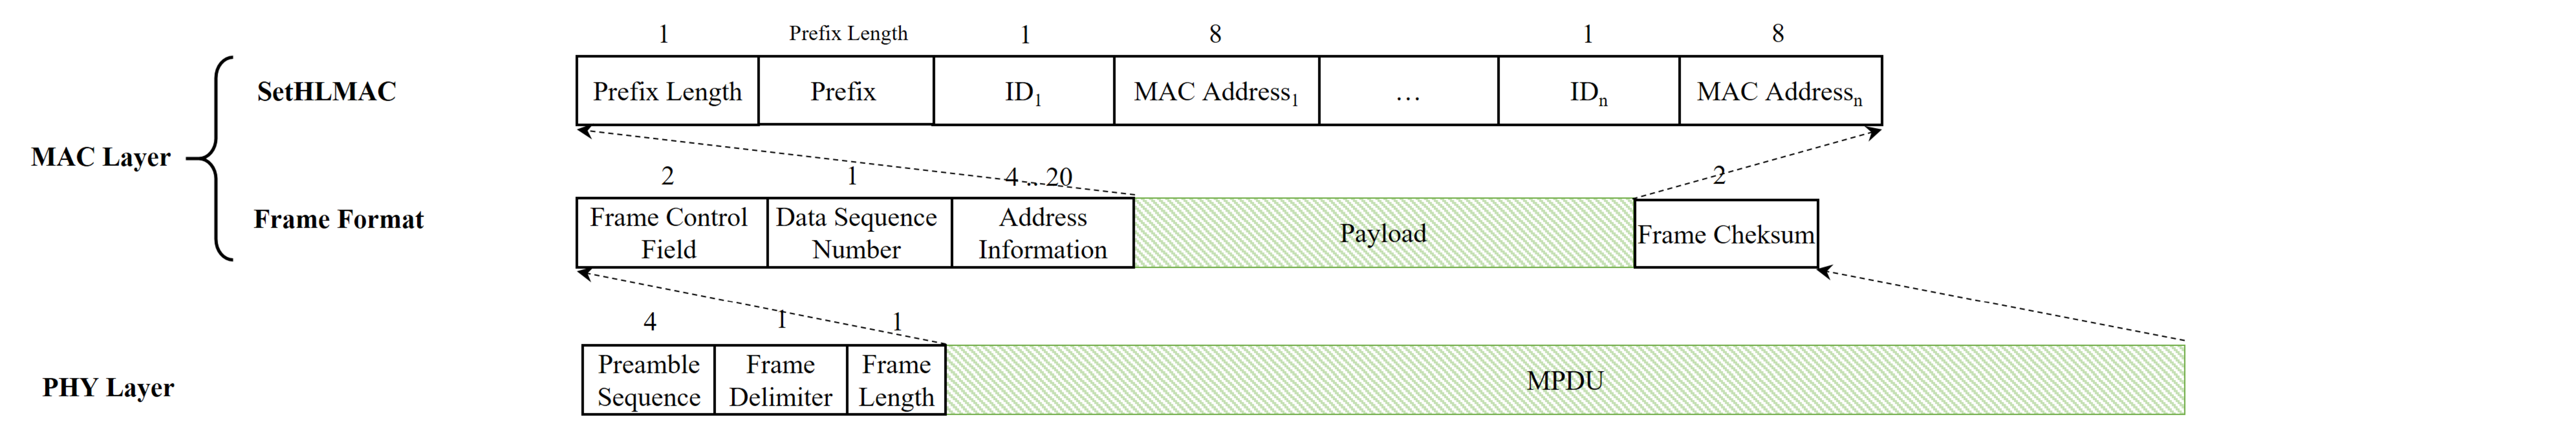
\includegraphics[width=\textwidth]{archivos/img/analisis/Comparation_frame_iotorii.eps}
    \caption{Mensajes de control en IoTorii \cite{rojas2021outperforming}}
    \label{fig:frameformat-setHLMAC}
\end{sidewaysfigure}


\subsubsection{Configuración del protocolo IoTorii}